\section{Implementierung}
Dieses Kapitel dient dazu nachzuvollziehen, wie sich das aus den zuvor beschriebenen Komponenten bestehende Programm, im Web verhalten würde. Um zu gewährleisten, dass das Programm bei Missverhalten keinen Schaden an dem gerade getesteten Forum anrichtet, werden ein eigenes Forum aufgebaut und ein vollständiger Arbeitszyklus lokal an diesem Forum getestet.

\subsection{Implementierungsumgebung}
Das Test-Forum muss Zugriff auf eine Datenbankquelle haben. Sie besteht für die Dauer der Tests aus einer Datenbank mit 50.000 Einträgen. Diese Einträge umfassen einen Beitragstitel, einen Beitragsinhalt und eine eindeutige Web-URL, die als ID benutzt wird. Die Beiträge sind in einer NoSQL-Datenbank `Elasticsearch` gespeichert. Sie bietet den Vorteil, dass mit nur einer Anfrage an die Datenbank in Beitragstitel und Beitragsinhalt, leicht nach einem bestimmten Suchwort gesucht werden kann und die ersten 20 gefundenen Beiträge zurückgeliefert werden.\\
Das Test-Forum wird lokal erstellt, um eine Vielzahl an Anfragen an ein im Internet verfügbares Forum zu vermeiden. Eine gewissenhafte Evaluierung könnte einem Internetforum eventuell durch zu viel Netzwerkverkehr schaden.\\
Geschrieben werden alle Programm mit Hilfe von `JavaScript`. Das Forum wird auf einem `Node.js-Server` laufen. 

\subsubsection{Aufbau des Forums}
Das Forum sollte einem originalen Internetforum möglichst nahe kommen, jedoch gleichzeitig eine Umgestaltung der einzelnen Seiten für Anmelden, Registrieren und Suchen nicht allzu aufwändig machen. Das erlaubt ein schnelles Debuggen, wenn das Programm falsche Daten für Registrierung, Login oder Suche extrahiert. Das Test-Forum umfasst eine Login-, eine Registrierungs- und eine Suchseite, auf die nach einem erfolgreichen Login redirected wird.

\subsubsection{Registrierung im Forum}

Die häufigste Registrierungsform, die man in diversen Internetforen findet, besteht aus 2 Feldern für das Passwort, 2 Feldern für die Email, einem Feld für den Nutzernamen und einer Checkbox, in der die Foren-AGB angenommen werden. Das wird durch das folgende Codebeispiel demonstriert.


\begin{figure}[h!]
\begin{lstlisting}[language=HTML5]
<form action="/reg" method="post">
Nutzername: <input type="text" name="fname"></br>
Email: <input type="text" name="email"></br>
Validate Email: 
<input type="text" name="re_email"></br>
Password: <input type="password" name="pwd"></br>
Validate Password: 
<input type="password" name="re_pwd"></br>
Accept AGB:<input type="checkbox" name="AGB"></br>
<input type="hidden" name="val1" value="val1">
<input type="hidden" name="val2" value="val2">
<input type="submit" value="Submit">
</form>
\end{lstlisting}
\caption{HTML-Code für die Erstellung einer Registrierungsseite mit Nutzernamen, Email- und Passwordfeldern sowie Checkbox}
\end{figure}

Aus Abbildung 2 ist leicht zu evaluieren, ob der Registrierungsprozess erfolgreich sein wird. Zu erwarten wäre ein `POST-Request` an die Toplevel-Domain + Formaction mit den POST-Parametern `fname`, `email`, `re\_email`, `pwd`,\\ `re\_pwd`, `AGB`, sowie den hidden Key-Value-Paaren, `val1 = hiddenvalue1` und `val2 = hiddenvalue2`.\\
In die POST-Parameter sollten die entsprechenden Felder `fname`, `email` und `pwd` jeweils der Name, die Email und das Passwort eingetragen sowie in den `re\_email`, `re\_pwd` jeweils die Email und das Passwort wiederholt und bestätigt werden.\\
Ist der HTTP-Server gestartet wird die Registrierungsseite analysiert und der folgende Request an den Server gesendet :

\begin{figure}[ht]
\begin{lstlisting}[language=HTML5]
http://localhost:12345/reg
{ val2: 'hiddenvalue2',
val1: 'hiddenvalue1',
AGB: 'on',
re_pwd: 'AjZt198#ev',
pwd: 'AjZt198#ev',
re_email: 'jpm96353@adiaq.com',
email: 'jpm96353@adiaq.com',
fname: 'Dominik' }
verification email to : jpm96353@adiaq.com
\end{lstlisting}
\caption{Inhalt des POST-Requests, den das Programm an das Forum bei einem Registrierungsaufruf sendet}
\end{figure}

Zu beachten ist, dass sich das Programm eine eigene Email angelegt hat. Sie stammt von der Internetseite `10minutemail`\footnote{https://10minutemail.net/ besucht: 10.06.2015}.
Diese Internetseite stellt für 10 Minuten eine kostenlose Email-Adresse zur Verfügung, mit der Emails empfangen und gesendet werden können. Die Registrierungsaufforderung wurde an die richtige URL des Servers gesendet, was aus dem `http://localhost:12345/reg` ersichtlich wird. Weiterhin sind alle erforderlichen Parameter des POST-Requests und auch die Wiederholungsfelder von Email und Passwort korrekt ausgefüllt worden. Die Checkbox für die AGB wurde angekreuzt und auch alle versteckten Input-Felder der Form sind mit übertragen. Insgesamt ist dieses eine gültige Registrierungsanfrage, die der Server mit einer Validierungs-Email an die angegebene Email-Adresse quittiert.

Das Programm überprüft alle 5 Sekunden, ob die Email eingegangen ist (Abbildung 4). Sollte dies der Fall sein, werden die Email analysiert und jeder darin befindliche Link aufgerufen. Ist innerhalb von 10 Minuten keine Email eingegangen, wird der Registrierungsversuch als gescheitert angesehen und das dem Nutzer mitgeteilt, denn die Email-Adresse ist nur 10 Minuten valide.

\begin{figure}[ht]
\begin{lstlisting}[language=HTML5]
registered
No new emails
No new emails
No new emails
location='readmail.html?mid=KfKcm0'
https://10minutemail.net/readmail.html?mid=KfKcm0
clicked: http://localhost:12345/validateUser?user=jpm96353@adiaq.com
\end{lstlisting}
\caption{Das Programm wartet auf Registrierungs-Email und ruft alle Links in der Email auf.}
\end{figure}

Der Validierungslink, den das Forum generiert und in der Email gesendet hat, wird aufgerufen (Abbildung 4) und der Validierungsversuch wird an das Forum gesendet, das den Nutzer als aktiven Nutzer validiert (Abbildung 5).

\begin{figure}[ht]
\begin{lstlisting}[language=HTML5]
/validateUser?user=jpm96353@adiaq.com
validate:
jpm96353@adiaq.com
\end{lstlisting}
\caption{Das Forum validiert den Nutzeraccount, da der Validierungslink bestätigt wurde.}
\end{figure}

Sollte der Registrierungsprozess nicht funktionieren, können die Registrierungsform nachgebaut und gegebenfalls Änderungen an den Feldbewertungsmetriken vorgenommen werden. Ein erneutes Testen kann erfolgen, ohne Webforen zu belasten. Es gibt für das Programm die Möglichkeit, den Registrierungsschritt zu überspringen. Wenn der Nutzer schon einen Nutzeraccount per Hand angelegt hat, kann er das dem Programm über Eingabeparameter mitteilen. Anstatt sich neu zu registrieren, nutzt es nun den vorhandenen Nutzeraccount. Damit kann, wenn die programmtechnische Registrierung fehlgeschlagen ist, trotzdem versucht werden, das Forum automatisch zu durchsuchen.

\subsubsection{Foren-Login}
Der Forenlogin sollte bei nicht angegebenen Logindaten mit den bei der Registrierung generierten Daten ausgeführt werden. Werden Accountdaten beim Programmstart angegeben sind, sollten diese auch benutzt werden. Der Loginrequest sollte drei Parameter enthalten, einmal den Nutzernamen, einmal das Passwort und eine Checkbox. Die Checkbox gibt an, ob man auf der Website eingeloggt bleiben möchte, um bei einem späteren Besuch nicht noch einmal die Nutzerdaten eingeben zu müssen. Das sind die gängigsten Login-Formulare, die im Internet existieren (Abbildung 6).

\begin{figure}[ht]
\begin{lstlisting}[language=HTML5]
<form action="/log" method="post">
Nutzername: 
<input type="text" name="fname"></br>
Password: 
<input type="password" name="pwd"></br>
Eingeloggt bleiben: 
<input type="checkbox" name="remember">
<input type="submit" value="Submit">
</form>
\end{lstlisting}
\caption{HTML-Code, der die Loginseite des Forums darstellt}
\end{figure}


\begin{figure}[h!]
\begin{lstlisting}[language=HTML5]
loginattempt: 
{fname:'Dominik',
remember: 'on',
pwd:'AjZt198#ev'}
\end{lstlisting}
\caption{Eingehende Loginanfrage des Programms im Forum}
\end{figure}

In Abbildung 7 ist zu sehen, dass alle erforderlichen Daten korrekt ausgefüllt wurden. Der Nutzername `Dominik` wurde, wie zu erwarten, als Wert des Feldes `fname` eingetragen. Die Checkbox wurde angekreuzt, das duch das `on` als Wert des Feldes `remember` deutlich wird. Das Passwort `AjZt198\#ev` wurde im richtigen Feld übermittelt.

Abbildung 8 zeigt, dass, wenn die Loginform Usernamen und Email abfragen sollte, ein valider Loginrequest abgesendet wird. Es sind sowohl Email als auch Nutzername korrekt ausgefüllt.

\begin{figure}[h!]
\begin{lstlisting}[language=HTML5]
loginattempt:
{email: 'jpm96353@adiaq.com',
fname: 'Dominik',
remember: 'on',
pwd: 'AjZt198#ev'}
\end{lstlisting}
\caption{Eingehende Loginanfrage des Programms im Forum mit Nutzername und Email}
\end{figure}

Auch etwaige versteckte Input-Felder werden korrekt gefunden und die Key-Value-Paare in dem POST-Request mit übergeben, was durch den Wert `v1` im Feld `hiddenvalue` sichtbar wird (Abbildung 9).

\begin{figure}[h!]
\begin{lstlisting}[language=HTML5]
loginattempt:
{email: 'jpm96353@adiaq.com',
fname: 'Dominik',
remember: 'on',
pwd: 'AjZt198#ev',
hiddenvalue: 'v1'}
\end{lstlisting}
\caption{Eingehende Loginanfrage des Clients im Forum mit versteckten Attributen}
\end{figure}


82 Loginseiten diverser im Internet gefundener Seiten wurden im händischen Test erfolgreich ausgefüllt und die zu erwartende Loginanfrage an den Server gesendet.\\
Es ist programmtechnisch möglich, sich in Foren automatisch zu registrieren und anzumelden. Im Folgenden müssen nach dem Loginvorgang nun noch relevante Beiträge zu den jeweiligen Firmenprodukten aus dem Forum extrahiert werden.\newline
In Internetforen werden Nutzer, die sich gerade angemeldet haben, auf die Hauptseite des Forums verwiesen. Damit der Browser das umsetzt, wird in der Antwort des Servers nach erfolgreichem Anmelden ein `Statuscode 302` gesendet. Dieser zeigt an, dass der Browser eine andere URL ohne das Zutun des Nutzers laden soll. Die URL steht im Location-Header der Antwort. Dieses muss programmtechnisch realisiert werden, da sonst, ohne den Redirect, bei einer Analyse des HTML-Quellcodes keine Suchform gefunden werden kann. Es würde immer die vorherige, also die Login-Seite analysiert werden.\\
Abbildung 10 zeigt einen Redirect nach einem erfolgreichen Login.

\begin{figure}[ht]
\begin{lstlisting}[language=HTML5]
successfull login from: jpm96353@adiaq.com
send 302 to redirect to /main
http://localhost:12345/main
\end{lstlisting}
\caption{Erfolgreicher Login im Forum und Redirect des Programms zur Hauptseite}
\end{figure}

Das Programm überprüft bei jeder Anfrage an den Server, ob der Statuscode sich von `200` (OK) unterscheidet. Sollte es wie in diesem Fall ein `302` (Redirect) sein, wird automatisch die neue URL mit einem GET-Request nachgeladen, damit im nächsten Schritt das neue HTML analysiert werden kann. In diesem Fall wird die Hauptseite des Forums als Nächstes geladen.
\newpage

\subsubsection{Suchen im Forum}

\begin{figure}[ht]
\begin{lstlisting}[language=HTML5]
http://localhost:12345/log
{ email: 'jpm96353@adiaq.com',
fname: 'Dominik',
pwd: 'AjZt198#ev',
hiddenvalue: 'v1' }
redirected
redirecturl: /main
\end{lstlisting}
\caption{Das Programm folgt dem Redirect auf die Hauptseite des Forums}
\end{figure}

Das Programm erkennt automatisch, dass er auf eine andere Seite verwiesen wurde und lädt diese (Abbildung 11). Das ist daran zu erkennen, dass das HTML, das im nächsten Schritt analysiert wird, nicht mehr das Login-HTML ist.

\begin{figure}[h!]
\begin{lstlisting}[language=HTML5]
<form accept-charset="UTF-8" action="/search" class="js-site-search-form" data-global-search-url="/search" data-repo-search-url="" method="get">
<div style="margin:0;padding:0;display:inline">
<input name="utf8" type="hidden" value="true"></div>
<input type="text" class="js-site-search-focus chromeless-input" data-hotkey="s" name="q" placeholder="Search OwnForum" data-global-scope-placeholder="Search OwnForum" data-repo-scope-placeholder="Search" tabindex="1" autocapitalize="off">
</form>
\end{lstlisting}
\caption{Zu analysierendes HTML nach dem Redirect enthält die Suchform}
\end{figure}

Das HTML aus Abbildung 12 wird nach einer Suchform durchsucht. Diese befindet sich meist in einer `GET-Form`. Da der Request ein `GET-Request` ist, wird das Suchwort in der URL codiert. Der Name des Key-Value-Paares, das für die Übermittlung zuständig ist, wird aus den Input-Feldern der Form generiert. Dieses Attribut hat meist in den Namen `q` oder `search`. Das Programm findet diese Suchform (Abbildung 13) und sendet die Suchanfrage an den Server.


\begin{figure}[ht]
\begin{lstlisting}[language=HTML5]
{ action: '/search', name: 'q' }
\end{lstlisting}
\caption{Vom Programm analysierte Suchform, gefundener Name des Suchparameters und die Such-URL}
\end{figure}


\begin{figure}[ht]
\begin{lstlisting}[language=HTML5]
/search?q=CRM
/search?q=LVM
/search?q=HCM
/search?q=ECOM
\end{lstlisting}
\caption{Eingehende Suchanfragen im Forum }
\end{figure}
Im Forum geht eine valide Suchanfrage ein (Abbildung 14).
Sollte das Suchwort im Titel oder im Beitragsinhalt vorkommen, wird der Link zu diesem Beitrag zurückgegeben. Dieser Link ist in dem Testforum eine eindeutige ID. Es ist anzunehmen, dass die Links in jedem Internetforum eine eindeutige ID für jeden Beitrag darstellen, da sie auf genau eine feste Internetadresse verweisen. So wie in einem Internetforum werden pro Suchwort die ersten 20 Treffer zu diesem Suchwort auf einer HTML-Seite zusammengefasst und ausgeliefert. Das Programm speichert alle Links und vermerkt, wie oft der Link bei unterschiedlichen Suchworten von dem Forum zurückgegeben wurde. Dazu wird das HTML nach allen vorkommenden Links durchsucht. Des Weiteren sollten Links entfernt werden, die in mehr als der Hälfte der Suchanfragen zu finden sind, da es sich hierbei meist um statische Links handelt, wie neueste Beiträge oder Links in den Navigationsleisten.
\newpage

\begin{figure}[h!]
\begin{lstlisting}[language=JavaScript]
dispatcher.onGet("/search", function(req, res) {
res.writeHead(200, {'Content-Type': 'text/html'})
var results = searchDataBaseForWord(req.params.q)
.then(function(results){
if(results.length > 0){
var temp = ''
for (var i = results.length - 1; i >= 0; i--) {
temp += '<a href="/'+ results[i] +'">Link</a>'
temp += '</br>'
}
temp +='<a href="/removeLink">REMOVELINK</a>'
temp += '</br>'
res.write(temp)
}else{
var temp = ''
temp +='<a href="/removeLink">REMOVELINK</a>'
temp += '</br>'
temp += "<h1> No valid Data found </h1>"
res.write(temp)
}
res.end() 
}) 
})
\end{lstlisting}
\caption{Erstellung der Ergebnisseite auf eine Suchanfrage im Forum}
\end{figure}

Für jede Suchanfrage das HTML erstellt, das die Links zu den jeweiligen passenden Dokumenten enthält (Abbildung 15). Diese Links stammen aus der Datenbankabfrage mit dem entsprechenden Suchwort.
Ein statischer Link, der wiederum die statischen Links auf Internetseiten simulieren soll, wird platziert. Er sollte danach vom Programm wieder entfernt werden, da er in mehr als der Hälfte der Anfragen vorhanden ist und somit wahrscheinlich keinen Link zu einem Beitrag darstellt.

\begin{figure}[h!]
\begin{lstlisting}[language=HTML5]
/search?q=besiege
/search?q=briar
/search?q=individuals
/search?q=evacuate
/search?q=steals
/search?q=detrimental
/search?q=untimely
/search?q=bestir
/search?q=graphical
/search?q=revelation
\end{lstlisting}
\caption{10 Suchanfragen des Programms an das Forum mit zufälligen Wörtern}
\end{figure}

\begin{figure}[h!]
\begin{lstlisting}[language=HTML5]
{"href=\"/g-1814892-S-5993338243263848452\"":1,
"href=\"/g-1850237-S-6005730948694503428\"":1,
"href=\"/g-115178-S-5999229826848821253\"":1,
"href=\"/g-66325-S-6001320511865446402\"":1,
"href=\"/g-66325-S-6003599070168440836\"":1,
"href=\"/g-54723-S-5999922118567956482\"":1}
\end{lstlisting}
\caption{Gesammelte Dokumente des Programms auf die 10 Suchanfragen}
\end{figure}

Bei 10 Suchanfragen (Abbildung 16) mit zufälligen englischen Wörtern an das Forum wurden 6 Dokumente in der Testdatenbank gefunden (Abbildung 17). Keines wurde doppelt getroffen und der statische Link wurde entfernt. Die Beiträge können nun mit einem `GET-Request` an den entsprechenden Link heruntergeladen und indiziert werden.
\newpage

\begin{figure}[h!]
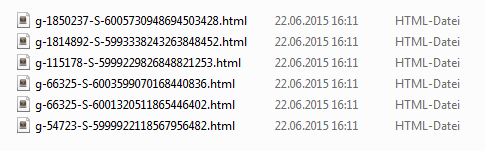
\includegraphics{./images/postdownload.png}
\caption{Heruntergeladene HTML-Seiten von Beiträgen der Suchanfragen}
\end{figure}


Es wurden erfolgreich die 6 Dokumente heruntergeladen, die das Forum auf die 10 Suchanfragen ausgeliefert hat (Abbildung 18).
Damit ist gezeigt, dass es möglich ist, sich automatisch in Foren zu registrieren, einzuloggen und nach bestimmten (firmenspezifischen) Schlagworten für Produkte zu suchen.
\newpage


